{\tt Detectors:} Detectors included in the calculation = {\tt ['SP', 'SP2', 'DP', 'PDVD', 'HD', 'VD', 'ND']} \\
{\tt Cap:} Cap on Raw data/year in PB = {\tt 30} \\
{\tt Base-Memory:} MB of memory per slot assumed as the average = {\tt 2000} \\
{\tt MaxYear:} Plot until year = {\tt 2026} \\
{\tt MinYear:} Plot starting with year = {\tt 2020} \\
{\tt Reprocess:} Number of years of data reprocessed when doing a new pass = {\tt {'SP': 3, 'DP': 2, 'SP2': 4, 'PDVD': 4, 'ProtoDUNEs': 3, 'VD': 100, 'HD': 100, 'FDs': 100, 'ND': 100, 'MARS': 1}} \\
{\tt PatternFraction:} Fraction of time taken in pattern recognition = {\tt {'SP': 0.7, 'SP2': 0.7, 'DP': 0.7, 'PDVD': 0.7, 'ProtoDUNEs': 0.7, 'HD': 0.1, 'VD': 0.1, 'FDs': 0.1, 'ND': 0.9, 'MARS': 0}} \\
{\tt TapeLifetimes:} Number of years kept on tape = {\tt {'Raw-Store': 100, 'Test': 0.5, 'Reco-Data-Store': 15, 'Sim-Store': 15}} \\
{\tt DiskLifetimes:} Number of years kept on disk = {\tt {'Raw-Store': 1, 'Test': 0.5, 'Reco-Data-Store': 2, 'Sim-Store': 2}} \\
{\tt TapeCopies:} Number of copies kept on tape = {\tt {'Raw-Store': 2, 'Test': 1, 'Reco-Data-Store': 1, 'Sim-Store': 1}} \\
{\tt DiskCopies:} Number of copies kept on disk = {\tt {'Raw-Store': 1, 'Test': 1, 'Reco-Data-Store': 2, 'Sim-Store': 1.5}} \\
{\tt PerYear:} Number of reprocessing done per year = {\tt {'Raw-Store': 1, 'Test': 1, 'Reco-Data-Store': 1, 'Sim-Store': 1, 'Events': 1, 'Sim-Events': 1, 'Reco-Data-CPU': 1, 'Sim-CPU': 1, 'Analysis': 1, 'Analysis-CPU': 1}} \\
{\tt Cores:} Description of cores, efficiency and speed relative to 2020 vintage = {\tt {'Efficiency': 0.7, '2020Units': 1}} \\
{\tt kHEPSPEC06PerCPU:} kHEPSPEC06 per core assumed = {\tt 0.011} \\
{\tt SplitsYear:} Year CERN no longer responsible for disk or tape = {\tt 2027} \\
{\tt SplitsEarly:} Division between FNAL/CERN/National for storage until SplitsYear = {\tt {'Tape': {'Raw-Store': {'FNAL': 0.5, 'CERN': 0.5, 'National': 0.0}, 'Sim-Store': {'FNAL': 1.0, 'CERN': 0.0, 'National': 0.0}, 'Reco-Data-Store': {'FNAL': 1.0, 'CERN': 0.0, 'National': 0.0}, 'Test': {'FNAL': 0.5, 'CERN': 0.5, 'National': 0.0}}, 'Disk': {'Raw-Store': {'FNAL': 0.5, 'CERN': 0.5, 'National': 0.0}, 'Sim-Store': {'FNAL': 0.25, 'CERN': 0.0, 'National': 0.75}, 'Reco-Data-Store': {'FNAL': 0.25, 'CERN': 0.0, 'National': 0.75}, 'Test': {'FNAL': 0.5, 'CERN': 0.5, 'National': 0.0}}}} \\
{\tt SplitsLater:} Division between FNAL/CERN/National for storage after SplitsYear = {\tt {'Tape': {'Raw-Store': {'FNAL': 0.5, 'CERN': 0.0, 'National': 0.5}, 'Sim-Store': {'FNAL': 0.5, 'CERN': 0.0, 'National': 0.5}, 'Reco-Data-Store': {'FNAL': 0.5, 'CERN': 0.0, 'National': 0.5}, 'Test': {'FNAL': 0.5, 'CERN': 0.0, 'National': 0.5}}, 'Disk': {'Raw-Store': {'FNAL': 1.0, 'CERN': 0.0, 'National': 0.0}, 'Sim-Store': {'FNAL': 0.25, 'CERN': 0.0, 'National': 0.75}, 'Reco-Data-Store': {'FNAL': 0.25, 'CERN': 0.0, 'National': 0.75}, 'Test': {'FNAL': 0.5, 'CERN': 0.0, 'National': 0.5}}}} \\
{\tt filename:} Input configuration file = {\tt MoreSim\_2022-11-21-2040.json} \\
\begin{figure}[h]
\centering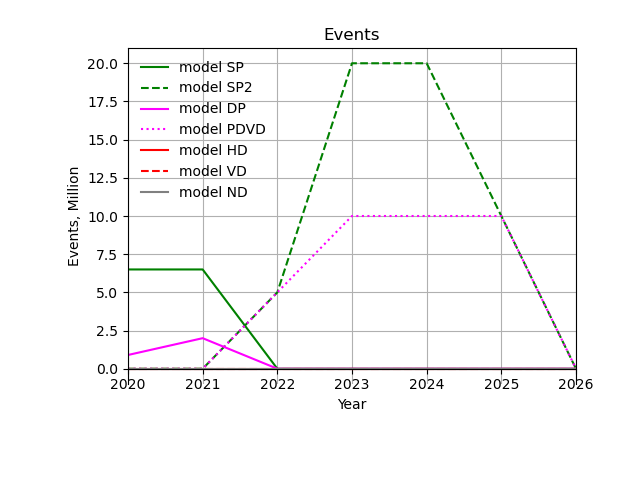
\includegraphics[height=0.4\textwidth]{MoreSim_2022-11-21-2026/MoreSim_2022-11-21-2026-Events.png}
\csvautotabularright{MoreSim_2022-11-21-2026/MoreSim_2022-11-21-2026-Events.csv}\caption{Projected million of detector events per year.  Reconstructed data resources are based on this number.}
\label{fig:Events}
\end{figure}
\begin{figure}[h]
\centering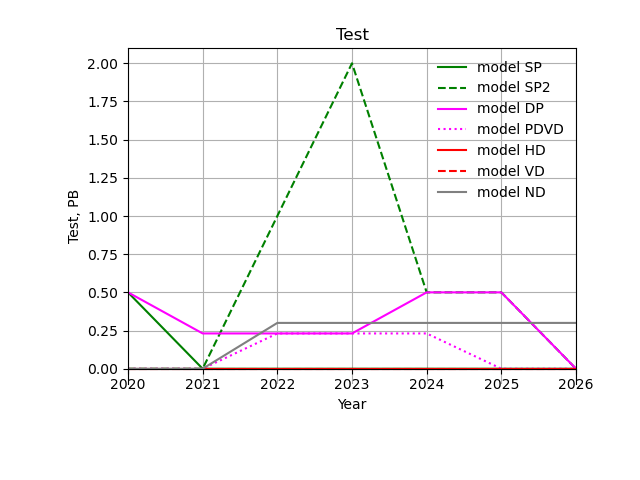
\includegraphics[height=0.4\textwidth]{MoreSim_2022-11-21-2026/MoreSim_2022-11-21-2026-Test.png}
\csvautotabularright{MoreSim_2022-11-21-2026/MoreSim_2022-11-21-2026-Test.csv}\caption{Projected PB of Test data per year.}
\label{fig:Test}
\end{figure}
\begin{figure}[h]
\centering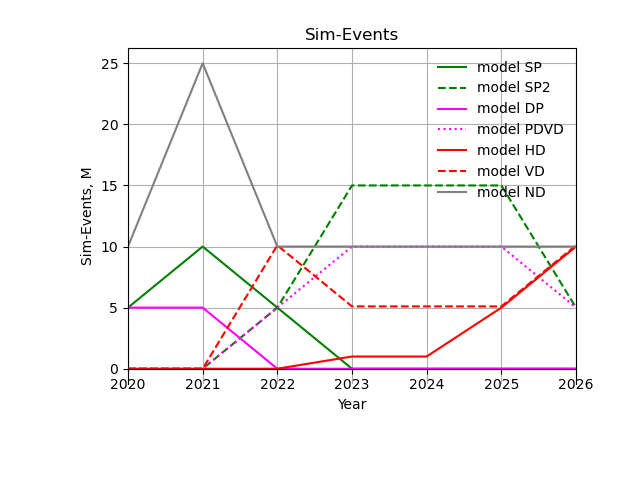
\includegraphics[height=0.4\textwidth]{MoreSim_2022-11-21-2026/MoreSim_2022-11-21-2026-Sim-Events.png}
\csvautotabularright{MoreSim_2022-11-21-2026/MoreSim_2022-11-21-2026-Sim-Events.csv}\caption{Projected millions of simulated events per year. Simulated data resources are based on this number. }
\label{fig:Sim-Events}
\end{figure}
\begin{figure}[h]
\centering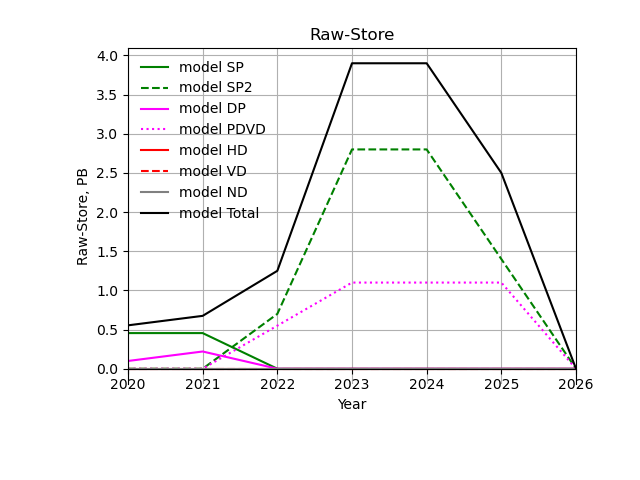
\includegraphics[height=0.4\textwidth]{MoreSim_2022-11-21-2026/MoreSim_2022-11-21-2026-Raw-Store.png}
\csvautotabularright{MoreSim_2022-11-21-2026/MoreSim_2022-11-21-2026-Raw-Store.csv}\caption{Projected raw data written per year in PB, derived from the number of events.}
\label{fig:Raw-Store}
\end{figure}
\begin{figure}[h]
\centering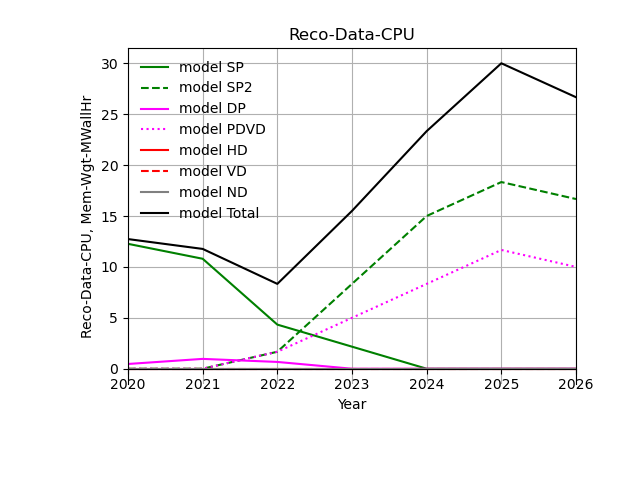
\includegraphics[height=0.4\textwidth]{MoreSim_2022-11-21-2026/MoreSim_2022-11-21-2026-Reco-Data-CPU.png}
\csvautotabularright{MoreSim_2022-11-21-2026/MoreSim_2022-11-21-2026-Reco-Data-CPU.csv}\caption{Projected CPU needs in core-years for data reconstruction.              Slot weighted wall time takes into account memory use and an efficiency correction.  Assumes rereconstruction of several years of older data.}
\label{fig:Reco-Data-CPU}
\end{figure}
\begin{figure}[h]
\centering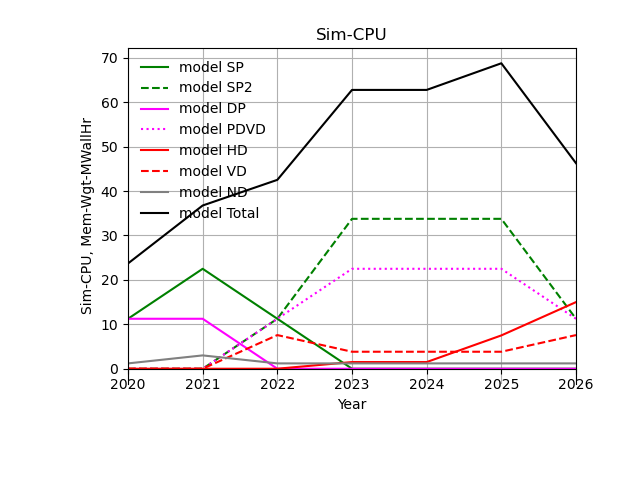
\includegraphics[height=0.4\textwidth]{MoreSim_2022-11-21-2026/MoreSim_2022-11-21-2026-Sim-CPU.png}
\csvautotabularright{MoreSim_2022-11-21-2026/MoreSim_2022-11-21-2026-Sim-CPU.csv}\caption{Projected CPU needs in core-years for simulation and reconstruction.              Slot weighted wall time takes into account memory use and an efficiency correction. Based directly on the number of simulated Events.}
\label{fig:Sim-CPU}
\end{figure}
\begin{figure}[h]
\centering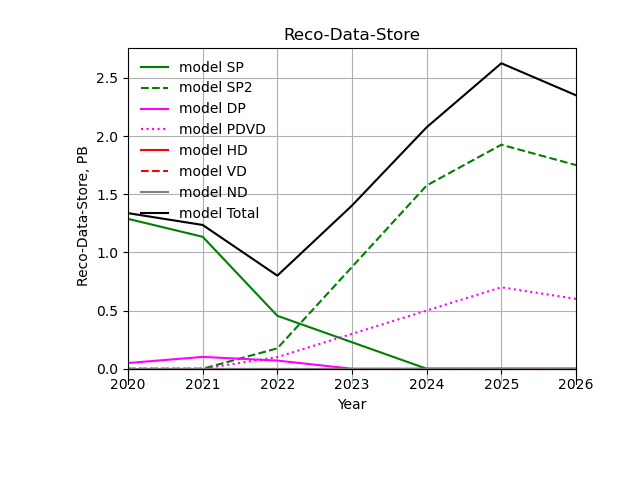
\includegraphics[height=0.4\textwidth]{MoreSim_2022-11-21-2026/MoreSim_2022-11-21-2026-Reco-Data-Store.png}
\csvautotabularright{MoreSim_2022-11-21-2026/MoreSim_2022-11-21-2026-Reco-Data-Store.csv}\caption{Projected PB of reconstructed data per year. Includes reprocessing.}
\label{fig:Reco-Data-Store}
\end{figure}
\begin{figure}[h]
\centering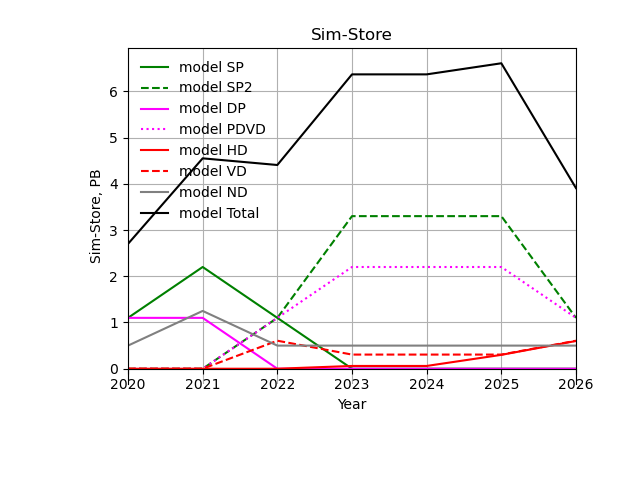
\includegraphics[height=0.4\textwidth]{MoreSim_2022-11-21-2026/MoreSim_2022-11-21-2026-Sim-Store.png}
\csvautotabularright{MoreSim_2022-11-21-2026/MoreSim_2022-11-21-2026-Sim-Store.csv}\caption{Projected PB of simulated data/year}
\label{fig:Sim-Store}
\end{figure}
\begin{figure}[h]
\centering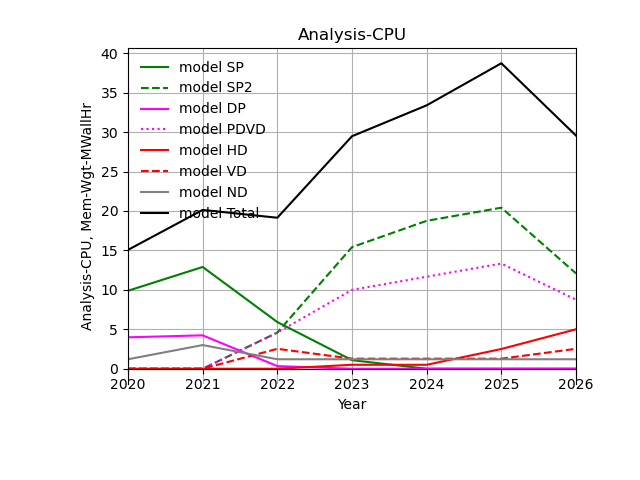
\includegraphics[height=0.4\textwidth]{MoreSim_2022-11-21-2026/MoreSim_2022-11-21-2026-Analysis-CPU.png}
\csvautotabularright{MoreSim_2022-11-21-2026/MoreSim_2022-11-21-2026-Analysis-CPU.csv}\caption{Slot weighted analysis CPU needs in core-years. Assumed to be a weighted fraction of reco+sim needs.}
\label{fig:Analysis-CPU}
\end{figure}
\begin{figure}[h]
\centering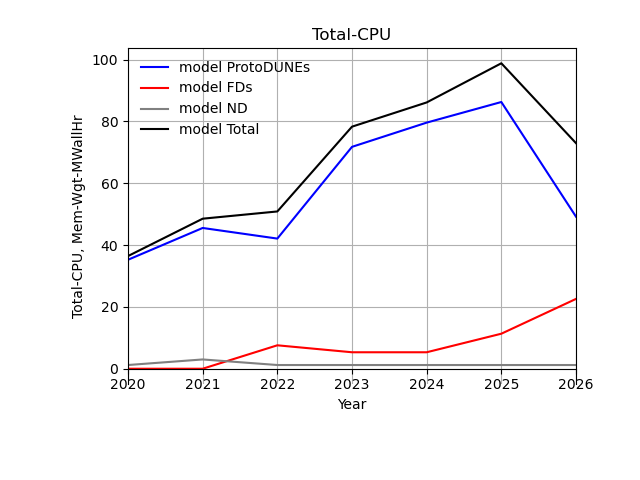
\includegraphics[height=0.4\textwidth]{MoreSim_2022-11-21-2026/MoreSim_2022-11-21-2026-Total-CPU.png}
\csvautotabularright{MoreSim_2022-11-21-2026/MoreSim_2022-11-21-2026-Total-CPU.csv}\caption{Slot weighted CPU needs in core-years. Slot weighted wall time takes into account memory and efficiency.}
\label{fig:Total-CPU}
\end{figure}
\begin{figure}[h]
\centering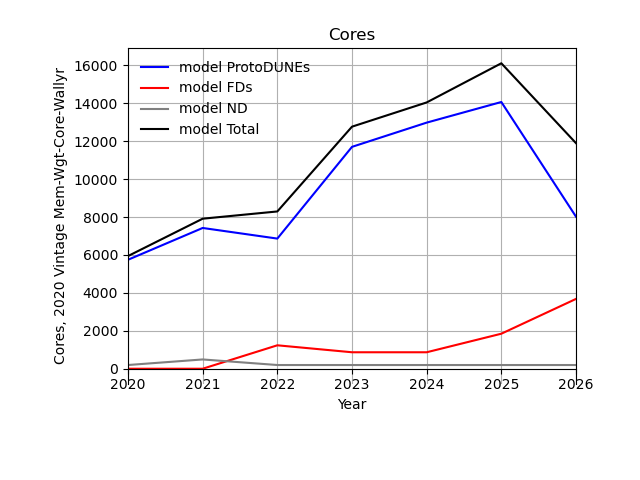
\includegraphics[height=0.4\textwidth]{MoreSim_2022-11-21-2026/MoreSim_2022-11-21-2026-Cores.png}
\csvautotabularright{MoreSim_2022-11-21-2026/MoreSim_2022-11-21-2026-Cores.csv}\caption{Slot weighted CPU needs in number of cores. Slot weighted wall time takes into account memory and efficiency.}
\label{fig:Cores}
\end{figure}
\begin{figure}[h]
\centering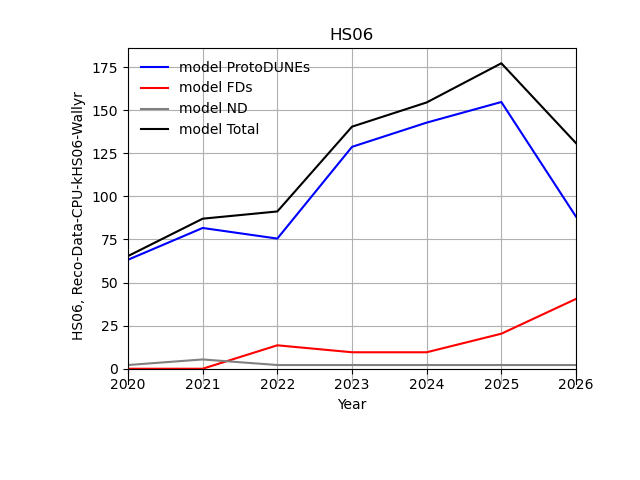
\includegraphics[height=0.4\textwidth]{MoreSim_2022-11-21-2026/MoreSim_2022-11-21-2026-HS06.png}
\csvautotabularright{MoreSim_2022-11-21-2026/MoreSim_2022-11-21-2026-HS06.csv}\caption{Slot weighted CPU needs in kHS06 hrs. Slot weighted wall time takes into account memory and efficiency.}
\label{fig:HS06}
\end{figure}
